% figures/sim-components_6.tex -- Figure 1 do ms_6.tex (E5b, 2026-10-12), o lugar de
% figures/sim-components.tex da k = 5. A figura e figures/sim-components.pdf, gerada por
% figures/make-sim-components.R dos curves.csv da E4.4 (so na desktop; SHA-256 no
% results/README.md): as medianas ponto a ponto das 100 replicas, numa grade comum. A
% opcao com as faixas vai ao supp (Figure S1), a da replica de ISE mediano foi descartada
% (escolha do autor, E5b). Legivel em preto e branco, sem cor na legenda (SS).
% \color{colR1} dentro do float (D75(d)).
\begin{figure}[t]
\color{colR1}
\centering
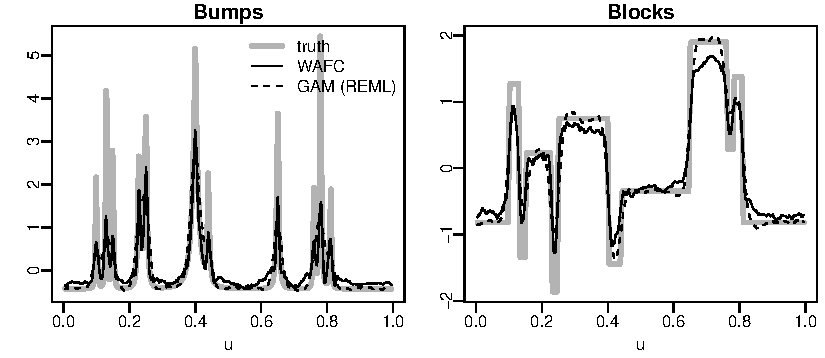
\includegraphics[width=\textwidth]{figures/sim-components.pdf}
\caption{Inhomogeneous cell, $n = 1000$: the components $\gcomp{1}{1}$
(bumps, left) and $\gcomp{1}{2}$ (blocks, right). The thick line is the
truth, and the solid and dashed lines are the pointwise medians over the 100
replicates of the WAFC and of GAM (REML); Figure~S1 of the Supplementary
Material adds the pointwise 5\% and 95\% quantiles.}
\label{fig:sim-components}
\end{figure}
